
%% bare_conf.tex
%% V1.3
%% 2007/01/11
%% by Michael Shell
%% See:
%% http://www.michaelshell.org/
%% for current contact information.
%%
%% This is a skeleton file demonstrating the use of IEEEtran.cls
%% (requires IEEEtran.cls version 1.7 or later) with an IEEE conference paper.
%%
%% Support sites:
%% http://www.michaelshell.org/tex/ieeetran/
%% http://www.ctan.org/tex-archive/macros/latex/contrib/IEEEtran/
%% and
%% http://www.ieee.org/

%%*************************************************************************
%% Legal Notice:
%% This code is offered as-is without any warranty either expressed or
%% implied; without even the implied warranty of MERCHANTABILITY or
%% FITNESS FOR A PARTICULAR PURPOSE! 
%% User assumes all risk.
%% In no event shall IEEE or any contributor to this code be liable for
%% any damages or losses, including, but not limited to, incidental,
%% consequential, or any other damages, resulting from the use or misuse
%% of any information contained here.
%%
%% All comments are the opinions of their respective authors and are not
%% necessarily endorsed by the IEEE.
%%
%% This work is distributed under the LaTeX Project Public License (LPPL)
%% ( http://www.latex-project.org/ ) version 1.3, and may be freely used,
%% distributed and modified. A copy of the LPPL, version 1.3, is included
%% in the base LaTeX documentation of all distributions of LaTeX released
%% 2003/12/01 or later.
%% Retain all contribution notices and credits.
%% ** Modified files should be clearly indicated as such, including  **
%% ** renaming them and changing author support contact information. **
%%
%% File list of work: IEEEtran.cls, IEEEtran_HOWTO.pdf, bare_adv.tex,
%%                    bare_conf.tex, bare_jrnl.tex, bare_jrnl_compsoc.tex
%%*************************************************************************

\documentclass[conference]{IEEEtran}
\usepackage{blindtext, graphicx}
\usepackage{listings}

\lstset{
    showstringspaces=false,
    backgroundcolor=\color{black!90},
    basicstyle=\lstfont{white},
    identifierstyle=\lstfont{white},
    keywordstyle=\lstfont{magenta!40},
    numberstyle=\lstfont{white},
    stringstyle=\lstfont{cyan},
    commentstyle=\lstfont{yellow!30},
    emph={
        hadoop, export
    },
    emphstyle={\lstfont{green!60!white}},
    breaklines=true
}


% correct bad hyphenation here
%\hyphenation{op-tical net-works semi-conduc-tor}


\begin{document}
%
% paper title
% can use linebreaks \\ within to get better formatting as desired
\title{MapReduce, Pig, HCatalog and Oozie:\\ A practical guide}


% author names and affiliations
% use a multiple column layout for up to three different
% affiliations
\author{\IEEEauthorblockN{Luis F. Rivera}
\IEEEauthorblockA{School of Engineering\\
Icesi University\\
Cali, Colombia\\
Email: lfrivera@icesi.edu.co}
}

% conference papers do not typically use \thanks and this command
% is locked out in conference mode. If really needed, such as for
% the acknowledgment of grants, issue a \IEEEoverridecommandlockouts
% after \documentclass

% for over three affiliations, or if they all won't fit within the width
% of the page, use this alternative format:
% 
%\author{\IEEEauthorblockN{Michael Shell\IEEEauthorrefmark{1},
%Homer Simpson\IEEEauthorrefmark{2},
%James Kirk\IEEEauthorrefmark{3}, 
%Montgomery Scott\IEEEauthorrefmark{3} and
%Eldon Tyrell\IEEEauthorrefmark{4}}
%\IEEEauthorblockA{\IEEEauthorrefmark{1}School of Electrical and Computer Engineering\\
%Georgia Institute of Technology,
%Atlanta, Georgia 30332--0250\\ Email: see http://www.michaelshell.org/contact.html}
%\IEEEauthorblockA{\IEEEauthorrefmark{2}Twentieth Century Fox, Springfield, USA\\
%Email: homer@thesimpsons.com}
%\IEEEauthorblockA{\IEEEauthorrefmark{3}Starfleet Academy, San Francisco, California 96678-2391\\
%Telephone: (800) 555--1212, Fax: (888) 555--1212}
%\IEEEauthorblockA{\IEEEauthorrefmark{4}Tyrell Inc., 123 Replicant Street, Los Angeles, California 90210--4321}}




% use for special paper notices
%\IEEEspecialpapernotice{(Invited Paper)}




% make the title area
\maketitle


\begin{abstract}
My abstract.
\end{abstract}
% IEEEtran.cls defaults to using nonbold math in the Abstract.
% This preserves the distinction between vectors and scalars. However,
% if the journal you are submitting to favors bold math in the abstract,
% then you can use LaTeX's standard command \boldmath at the very start
% of the abstract to achieve this. Many IEEE journals frown on math
% in the abstract anyway.

% Note that keywords are not normally used for peerreview papers.
\begin{IEEEkeywords}
map reduce, pig, hive, hcatalog, oozie.
\end{IEEEkeywords}






% For peer review papers, you can put extra information on the cover
% page as needed:
% \ifCLASSOPTIONpeerreview
% \begin{center} \bfseries EDICS Category: 3-BBND \end{center}
% \fi
%
% For peerreview papers, this IEEEtran command inserts a page break and
% creates the second title. It will be ignored for other modes.
\IEEEpeerreviewmaketitle



\section{Introduction}
\textit{Apache Hadoop} es un \textit{framework} de código abierto para el almacenamiento y procesamiento de grandes volúmenes de datos \footnote{https://hortonworks.com/apache/hadoop/}. Generalmente, Hadoop es considerado como un ecosistema, en el que habitan, entre otras, herramientas como \textit{Apache Hive}, \textit{Apache Pig}, y \textit{Apache Oozie}, las cuales fueron concebidas con el objetivo de complementar los cuatro elementos principales del core de Hadoop (HDFS, MapReduce, YARN, y Common)\footnote{http://www.bmc.com/guides/hadoop-ecosystem.html}. \\

El objetivo principal de este proyecto consiste en analizar un subconjunto de las herramientas pertenecientes al ecosistema de Hadoop, desde la perspectiva de la infraestructura computacional necesaria ponerlas en marcha y de los principales atributos de calidad involucrados en el uso de las mismas. Para este propósito, un escenario de pruebas controlado fue configurado usando la versión 5.10.1 de \textit{Cloudera Manager} (CDH 5.10.1). Dicha configuración fue establecida como se muestra en la figura \ref{deployment_diagram}

\begin{figure}[H]
\label{deployment_diagram}
  \centering
      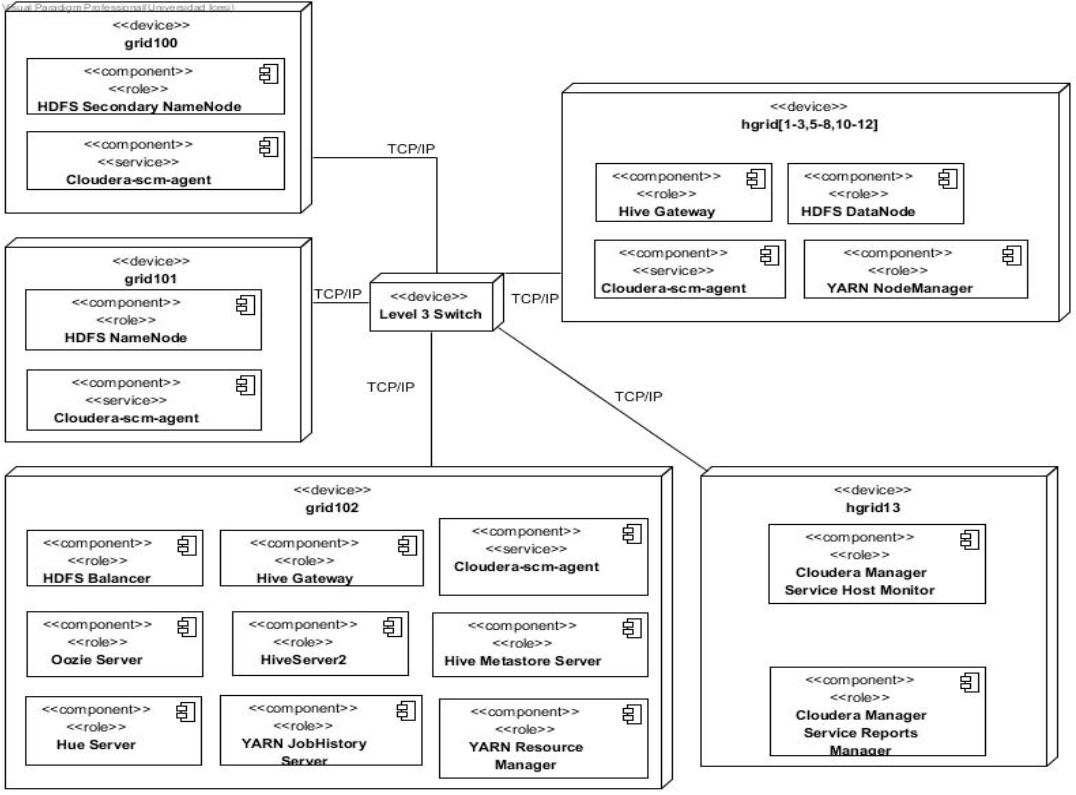
\includegraphics[width=\textwidth, height=2.5in]{fig/deployment}
  \caption{Diagrama de despliegue de la configuración de CDH 5.10.1 en el laboratorio \textit{LIASON} de la Universidad Icesi.}
\end{figure}

Cada uno de los casos de estudio de minería de datos presente en este proyecto se basa en los datos provistos por el \textit{National Climatic Data Center} (NCDC). Dichos datos son recolectados por medio de sensores climáticos, los cuales recolectan información cada hora, de forma diaria, en distintas estaciones a lo largo del mundo. Dichos datos se encuentran registrados a través de lineas en archivos de texto. La figura \ref{dataset} muestra la descripción del conjunto de datos mencionado previamente. \\

\begin{figure}[H]
\label{dataset}
  \centering
      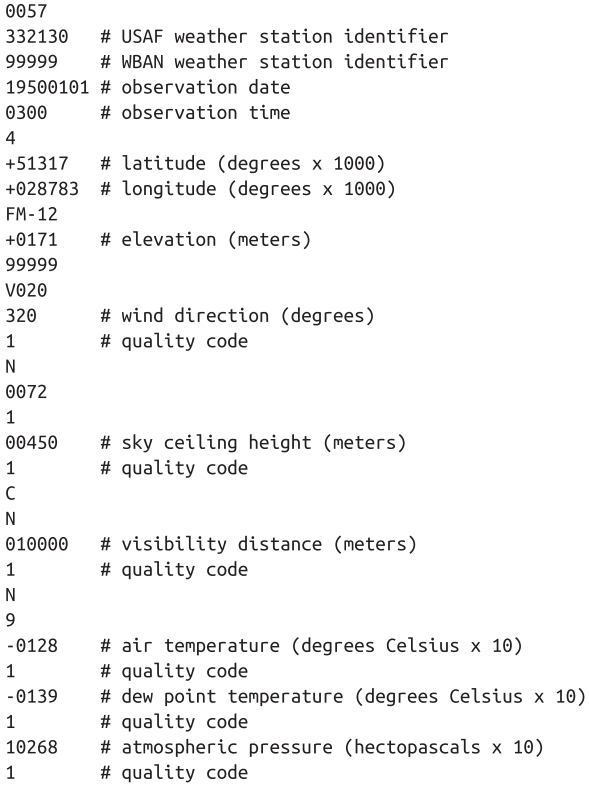
\includegraphics[width=\textwidth, height=3.5in]{fig/dataset}
  \caption{Descripción del conjunto de datos. Tomado de \cite{White:2012:HDG:2285539}}
\end{figure}

El resto del presente documento se encuentra distribuido como se muestra a continuación. En la sección 1 se describen formalmente el objetivo general y los objetivos objetivos específicos del proyecto. En la sección 2 se presentan los tipos de pruebas ejecutadas sobre las herramientas \textit{MapReduce}, \textit{Apache Pig}, y \textit{Apache Hive} para entender la diferencia entre los tiempos de ejecución de las mismas. En la sección 3 se ilustran las distintas pruebas llevadas a cabo sobre las herramientas \textit{Apache Pig} y \textit{HCatalog} para verificar la posibilidad de extender las funcionalidades y capacidades provistas por \textit{Pig}. En la sección 4 se detallan las pruebas realizadas sobre \textit{Apache Ooozie}, las cuales buscan evidenciar la re-usabilidad y mantenibilidad de las aplicaciones desarrolladas sobre esta herramienta. La sección 5 muestra los resultados de la ejecución de las pruebas descritas previamente. En la sección 6 se presentan las conclusiones del presente trabajo. Finalmente, la sección 7 muestra las posibilidades de trabajo futuro que se podrían desarrollar a partir de lo que aquí se presenta.

\section{MapReduce, Pig and Hive}
\subsection{Running MapReduce}


\subsection{Running Pig}

\subsection{Running Hive}

\section{Pig and HCatalog}
Pig and HCatalog.

\section{Oozie}
Oozie.

\section{Results}
Results.

\section{Conclusions}
Conclusions.

\section{Future work}
Future work.
% references section

% can use a bibliography generated by BibTeX as a .bbl file
% BibTeX documentation can be easily obtained at:
% http://www.ctan.org/tex-archive/biblio/bibtex/contrib/doc/
% The IEEEtran BibTeX style support page is at:
% http://www.michaelshell.org/tex/ieeetran/bibtex/
%\bibliographystyle{IEEEtran}
% argument is your BibTeX string definitions and bibliography database(s)
%\bibliography{IEEEabrv,../bib/paper}
%
% <OR> manually copy in the resultant .bbl file
% set second argument of \begin to the number of references
% (used to reserve space for the reference number labels box)
\begin{thebibliography}{1}

\bibitem{IEEEhowto:kopka}
H.~Kopka and P.~W. Daly, \emph{A Guide to \LaTeX}, 3rd~ed.\hskip 1em plus
  0.5em minus 0.4em\relax Harlow, England: Addison-Wesley, 1999.

\end{thebibliography}

% biography section
% 
% If you have an EPS/PDF photo (graphicx package needed) extra braces are
% needed around the contents of the optional argument to biography to prevent
% the LaTeX parser from getting confused when it sees the complicated
% \includegraphics command within an optional argument. (You could create
% your own custom macro containing the \includegraphics command to make things
% simpler here.)
%\begin{biography}[{\includegraphics[width=1in,height=1.25in,clip,keepaspectratio]{mshell}}]{Michael Shell}
% or if you just want to reserve a space for a photo:

\begin{IEEEbiography}[{\includegraphics[width=1in,height=1.25in,clip,keepaspectratio]{picture}}]{John Doe}
\blindtext
\end{IEEEbiography}

% You can push biographies down or up by placing
% a \vfill before or after them. The appropriate
% use of \vfill depends on what kind of text is
% on the last page and whether or not the columns
% are being equalized.

%\vfill

% Can be used to pull up biographies so that the bottom of the last one
% is flush with the other column.
%\enlargethispage{-5in}




% that's all folks
\end{document}


